% Drawing 85/05-5 -- folder 85, batch 05, archive page 92 (PDF page 93).
% Transcription: en haut à gauche, un petit dessin de tétraèdre : sommets $s$ (en haut) et $s'$ (à droite), l'arête de $s$ au sommet du bas au premier plan, la face de gauche hachurée de traits horizontaux, l'arête cachée au crayon
% Kind: tetrahedron with a hatched face. Method 2 (schematic redraw from the facsimile). Status: ok.
% Notes: Ink. Four vertices (dots at s and at the bottom vertex), the five visible edges, the hidden edge from the left vertex to s' in pencil; the left face hatched with horizontal strokes (six drawn for his seven or eight), light pencil hatching at the lower right. Redrawn 2026-11-12 (issue 128): to check again.
% Coordinates: 1 unit = 1 mm = 1/100 of the crop width (bbox in page fractions: [0.12, 0.08, 0.3, 0.2]).
% Redrawn by Claude (claude-fable-5-2), issue #128, 2026-11-12; not checked by a human; not compiled (no TeX in the session).
% Rights: reproduces part of the work -- behind RENDER_TRANSCRIPTS, never published by itself.
\documentclass[tikz,border=3pt]{standalone}
\usepackage{amsmath,amssymb}
\usetikzlibrary{patterns,arrows.meta}
\tikzset{pencil/.style={black!45}, struck/.style={black!35}, mpt/.style={circle,draw,inner sep=1.3pt}, pt/.style={circle,fill,inner sep=0.9pt}, opt/.style={circle,draw,fill=white,inner sep=1.1pt}}
\begin{document}
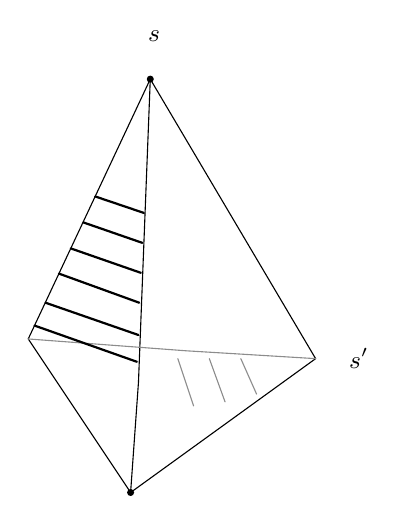
\begin{tikzpicture}[x=1mm,y=1mm,line cap=round,line join=round,font=\scriptsize]
\draw (52.5,-17.5) -- (37,-50.5) -- (50,-70) -- (73.5,-53) -- (52.5,-17.5);
\draw (52.5,-17.5) -- (51,-56) -- (50,-70);
\draw[pencil] (37,-50.5) -- (57,-52) -- (73.5,-53);
\node[pt] at (52.5,-17.5) {};
\node[pt] at (50,-70) {};
\draw[thick] (45.5,-32.4) -- (51.7,-34.5);
\draw[thick] (44,-35.7) -- (51.5,-38.3);
\draw[thick] (42.4,-39) -- (51.3,-42.1);
\draw[thick] (40.9,-42.2) -- (51.1,-45.9);
\draw[thick] (39.2,-45.9) -- (51,-50);
\draw[thick] (37.8,-48.8) -- (50.8,-53.4);
\draw[pencil] (56,-53) -- (58,-59);
\draw[pencil] (60,-53) -- (62,-58.5);
\draw[pencil] (64,-53) -- (66,-57.5);
\node[inner sep=1pt] at (53,-12) {\small $s$};
\node[inner sep=1pt] at (79,-53) {\small $s'$};
\end{tikzpicture}
\end{document}
